\chapter{RESULTADOS Y DISCUSIÓN}

\section{Resultados de Imagenes Recortadas}

\subsection{Resultados de Recorte por la Izquierda}

El procedimiento de realizar el recorte se explicó en el item 3.4.1. Los resultados obtenidos mediante esta técnica se muestra en la figura \ref{fig:left_use}.

\begin{figure}[!ht]
  \centering
  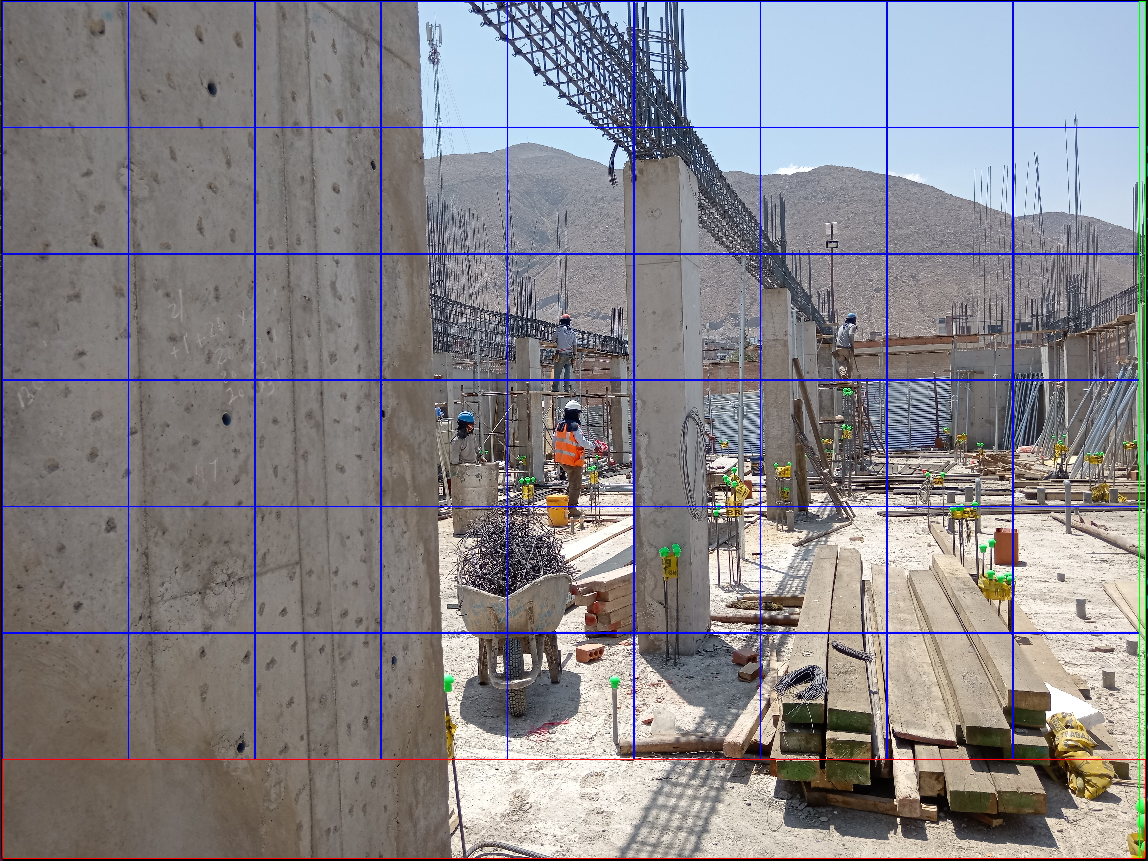
\includegraphics[width=.49\linewidth]{images/left_use.png}
  \caption{Ejemplo del resultado obtenido mediante el recorte por la izquierda.}
  \label{fig:left_use}
\end{figure}

\subsection{Resultados de Recorte Centrado}

Los resultados obtenidos mediante la técnica de recorte centrado se muestra en la siguiente figura \ref{fig:center_use}.

\begin{figure}[!ht]
  \centering
  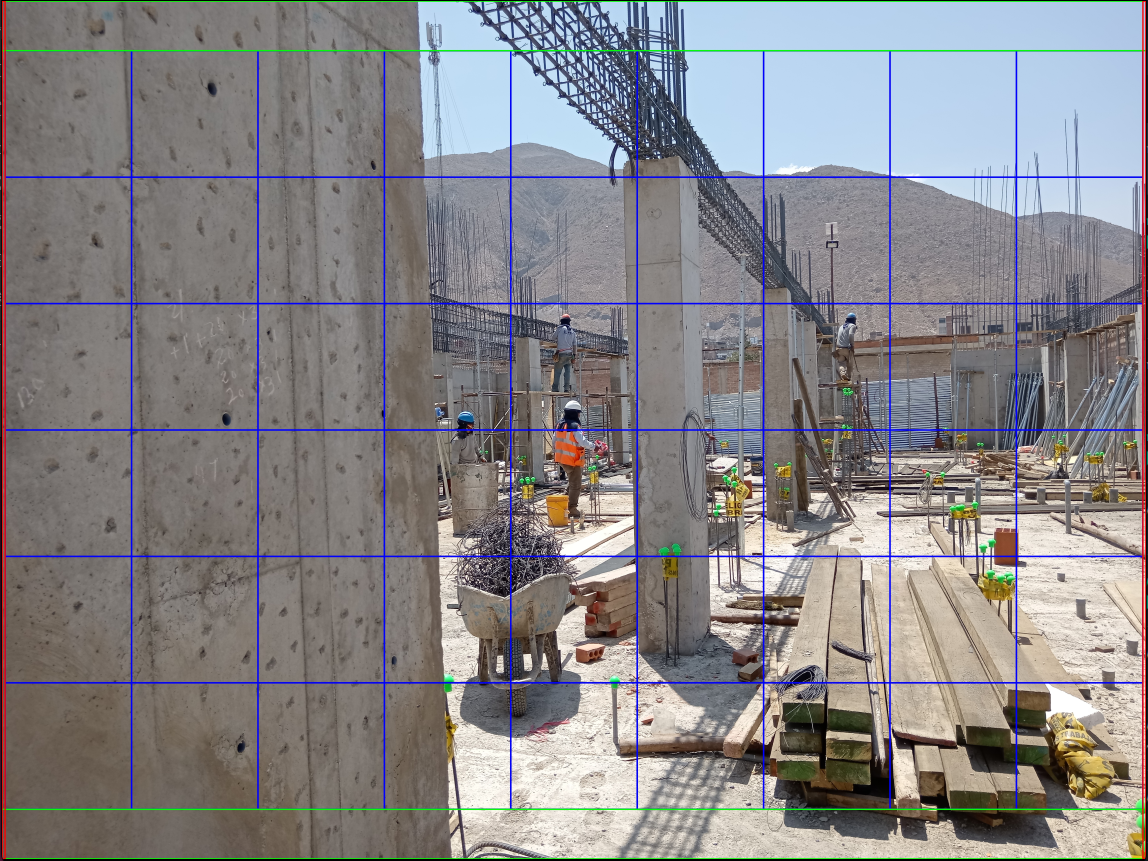
\includegraphics[width=.49\linewidth]{images/center_use.png}
  \caption{Ejemplo de resultado obtenido mediante el recorte centrado.}
  \label{fig:center_use}
\end{figure}

\subsection{Resultados de Recorte Superpuesto}

Los resultados obtenidos mediante la técnica de recorte superpuesto se muestra en la siguiente figura \ref{fig:full_use}.

\begin{figure}[!ht]
  \centering
  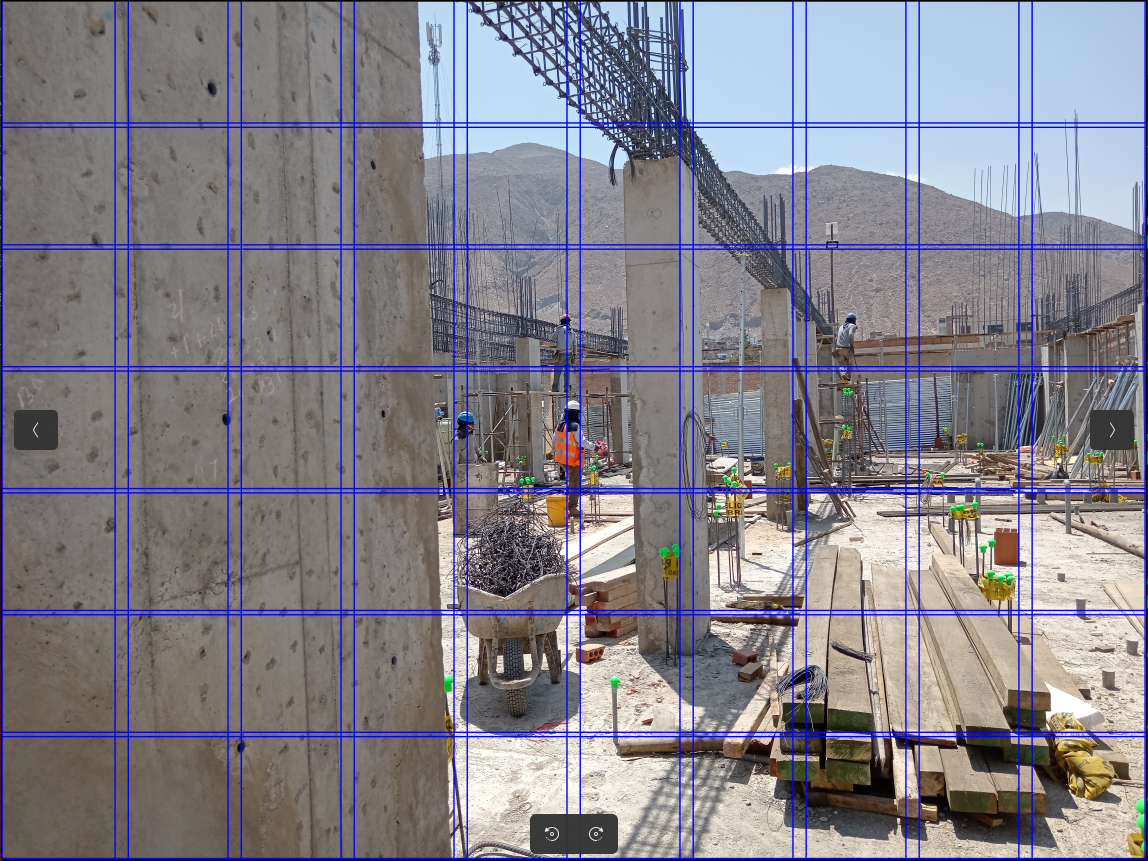
\includegraphics[width=.49\linewidth]{images/full_use.png}
  \caption{Ejemplo de resultado obtenido mediante el recorte superpuesto.}
  \label{fig:full_use}
\end{figure}

\subsection{Resultados de Recorte por Reconocimiento}

Los resultados obtenidos mediante la técnica de reconocimiento personas con el modelo preentrenado de yolov8m. El recorte se realizo a partir de la detección de las coordenadas de posición de la persona detectada, dandole las dimensiones de 640x640 pixles para el recorte.

\subsection{Resumen Segun las Técnicas de Recorte}

La siguiente tabla \ref{tab:summary_table} muestra el resultado de haber utilizado 4 técnicas de recorte de imagenes.

\begin{table}[ht]
  \centering
  \begin{tabular}{|l|c|c|}
      \hline
       & \textbf{Antes del filtro}  & \textbf{Despues del filtro}\\ \hline
      \textbf{Recorte por izquierda} & 3564 & 469 \\ \hline
      \textbf{Recorte centrado} & 3564 & 493 \\ \hline
      \textbf{Recorte superpuesto} & 4221 & 503 \\ \hline
      \textbf{Recorte con yolov8} & - & 289 \\ \hline
      \textbf{total} & \textbf{11349} & \textbf{1754} \\ \hline
  \end{tabular}
  \caption{Cantidad de imagenes después de aplicar las 4 técnicas de recorte antes del filtrado y después del filtrado.}
  \label{tab:summary_table}
\end{table}

\subsection{Resultado Final Obtenido}

El resultado final obtenido después de aplicar el primer filtro con la configuración por defecto del modelo  preentrenado yolov8m, el segundo filtro con un nivel de confianza del 90\% del modelo preentrenado yolov8x y finalmente la técnica de aumentacion de datos se muestra en el siguiente cuadro \ref{tab:final_report}.

\begin{table}[ht]
  \centering
  \begin{tabular}{|l|c|c|}
      \hline
       & \textbf{Total de imagenes} \\ \hline
      \textbf{Primer filtro} & 1754 \\ \hline
      \textbf{Segundo filtro} & 624 \\ \hline
      \textbf{Aumentación de datos} & 1248 \\ \hline
  \end{tabular}
  \caption{Cantidad de imágenes obtenidas despues de las técnicas de filtro y aumentación de datos.}
  \label{tab:final_report}
\end{table}

